% !TEX root=../main.tex
\section{Tutorial}
\subsection{Подробнее о циклах перестановок}
Модифицируем программу \ref{code:permutation_sample} так, чтобы она считала еще и циклы перестановок.
Это даст код \ref{code:permutation_sample_cycle}.

\pythonfile{../w7/programs_tutorial_7/permutation_sample_cycle}{Генерация перестановок и подсчет получающихся циклов (\texttt{permutation\_sample\_cycle.py})}{code:permutation_sample_cycle}

Важная часть здесь --- словарь \textit{cycle\_dict}, который ключу $k$ сопоставляет его партнера по перестановке.
Строки 15-23 мы уже знаем: они были в программе \ref{code:markov_harmonic_bosons} и считали циклы.
Строка 24 аккумулирует статистику по длинам циклов.

\subsection{Рекуррентное соотношение на число перестановок}
\begin{wrapfigure}[16]{r}{0.3\linewidth}
    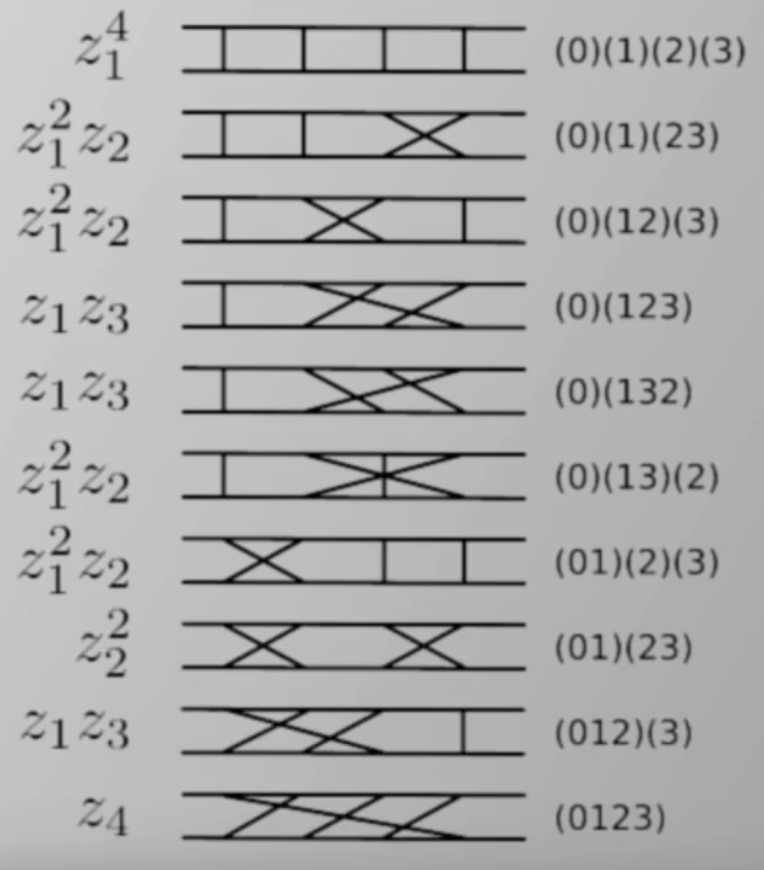
\includegraphics[width=\linewidth]{fig/permutations-weights}
    \caption{Различные циклы и их результирующие веса}
    \label{fig:permutations-weights}
\end{wrapfigure}
Рассмотрим 4 частицы и их $4!=24$ возможные перестановки.
Посчитаем для них функцию разбиения:
\begin{equation}
    \label{eq:Y_N-definition}
    Y_N = \sum\limits_{\text{permutations}}^{} \text{weight} (P)
\end{equation}

Дадим каждому циклу длиной $k$ вес $z_k$, т.е. цикл длиной 1 будет иметь вес $z_1$, цикл длиной 3 будет иметь вес $z_3$ и т.д.
Теперь <<разъединим>> последний элемент вместе с его циклом, разбив тем самым множество на две части.
Будем считать, что последний элемент вместе со своим циклом (будем называть такой цикл \textit{циклом последнего элемента}) имеют длину $k$, вес $z_k$ и содержит элементы $\{n_1, \dots, n_{k-1}, \text{last element}\}$ ($n_1$ не обязательно равно 1).

За бортом у нас останутся $N-k$ элементов с функцией разбиения $Y_{N-k}$.
Тогда для $Y_N$ можно записать:
\begin{align}
    \nonumber
    & Y_{N}=\sum_{k=1}^{N} z_{k}
    \underbrace{\left\{\begin{array}{c}\text { number of } \\ \text { choices for } \\ \left\{n_{1}, \ldots, n_{k-1}\right\}\end{array}\right\}}_{\left({}^{N-1}_{k-1}\right)=\frac{(N-1)!}{(k-1)!(N-k)!}}
    \underbrace{\left\{\begin{array}{c}\text { number of } \\ \text { cycles with } \\ \left\{n_{1}, \ldots, n_{k}\right\}\end{array}\right\}}_{(k-1)!}
    Y_{N-k} \\
    \label{eq:Y_N-recursion}
    & Y_N = \frac{1}{N} \sum_{k=1}^{N} z_{k} \frac{N !}{(N-k) !} Y_{N-k} \\
    & Y_0 = 1
\end{align}

Это рекуррентное соотношение позволяет подсчитать $Y_N$.

Если мы положим $z_i = 1$ для любого $i$, то получим уже знакомый случай.
Заметим, однако, что при такой подстановке выражение под суммой в \eqref{eq:Y_N-recursion} перестает зависеть от $k$.
Это означает, что последний элемент входит с равной вероятностью во все циклы длиной от 1 до $N$.

\subsection{Рекуррентное соотношение на статсумму}
\begin{wrapfigure}{r}{0.2\linewidth}
    \label{fig:cycle-0-1-23}
    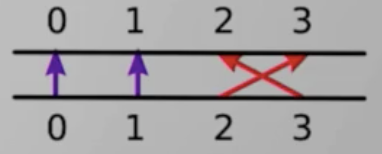
\includegraphics[width=\linewidth]{fig/cycle-0-1-23}
    \caption{Цикл ${\color{purple} (0)(1)} {\color{red} (23)}$}
\end{wrapfigure}
Мы уже знаем, что статсумму можно считать проще благодаря \eqref{eq:Z_0_132-full}.
Можем пойти дальше: обозначая одномерный интеграл за $z(\beta)$:
\begin{equation}
    \label{eq:z_beta-definition}
    z (\beta) = \int dx \rho(x, x, \beta)
\end{equation}
получим, например, $Z_{{\color{purple} (0)(1)} {\color{red} (23)}} = {\color{purple} z(\beta)^2} {\color{red} z(2\beta)}$ (цвета см. на картинке \ref{fig:cycle-0-1-23}).

Для гармонического осциллятора $z(\beta)$ известно \eqref{eq:upsilon-geometrical}:
\begin{align}
    \label{eq:z_small-3d-hamonic}
    & z(\beta) =\int d \mathbf{x} \rho(\mathbf{x}, \mathbf{x}, \beta) 
    = \left(\int d x \rho(x, x, \beta)\right) \left(\int d y \rho(y, y, \beta)\right) \left(\int d z \rho(z, z, \beta)\right) = \\
    & = \left(\sum_{E_{x}=0}^{\infty} e^{-\beta E_{x}}\right)\left(\sum_{E_{y}=0}^{\infty} e^{-\beta E_{y}}\right) \left(\sum_{E_{z}=0}^{\infty} e^{-\beta E_{z}}\right) 
    = \left(\frac{1}{1-e^{-\beta}}\right)^{3}
\end{align}

Для идеальных бозонов статсумма $N$ частиц разбивается на сумму произведений статсумм одной частицы:
\begin{align}
    \label{eq:Z-N_particle-ideal-bosons-strict}
    & Z_{N} = \frac{1}{N !} \sum_{P} Z_{P} & Z_{P} = \left\{\begin{array}{c}\text { product of } \\ \text { single-particle } \\ \text { partition functions }\end{array}\right\}
\end{align}

Но эту сумму сложно брать, поэтому предлагается другой путь.

Вспомним формулу \eqref{eq:Y_N-recursion}.
Для нее в качестве весов $z_k$ можно подставить $z(k\beta)$ из \eqref{eq:z_small-3d-hamonic}.
В самом деле, $z(k\beta)$ по построению представляет из себя вклад цикла длины $k$ в общую статсумму.
А сравнивая формулу для $Z_N$ \eqref{eq:Z-N_particle-ideal-bosons-strict} с формулой на $Y_N$ \eqref{eq:Y_N-recursion}, видим, что \eqref{eq:Z-N_particle-ideal-bosons-strict} сводится к \eqref{eq:Y_N-recursion} подстановкой $z_k=z(\beta)$ (при этом остальные множители в рекурсивной формуле на $Y_N$ не имеют отношению к весу перестановки).

Следующим шагом будет преобразование \eqref{eq:Y_N-recursion} (Landsberg, 1961):
\begin{align}
    \label{eq:Y_N-to-Z_N}
    \nonumber
    & Y_{N}=\frac{1}{N} \sum_{k=1}^{N} z_{k} \frac{N !}{(N-k) !} Y_{N-k} \\
    \nonumber
    & \boxed{\frac{Y_{N}}{N !}}=\frac{1}{N} \sum_{k=1}^{N} z_{k} \boxed{\frac{Y_{N-k}}{(N-k) !}} \\
    & Z_{N}=\frac{1}{N} \sum_{k=1}^{N} z_{k} Z_{N-k} \quad Z_0 = 1
\end{align}
Выделить $Z = \frac{Y_N}{N!}$ позволяет определение \eqref{eq:Z-N_particle-ideal-bosons-strict} и смысл $Y_N$.

Уравнение \eqref{eq:Y_N-to-Z_N} связывает статсумму системы $N$ идеальных бозонов с статсуммой системы $N-k$ идеальных бозонов и статсуммой одной частицы.
Это аналитическое решение реализовано в коде \ref{code:canonic_harmonic_recursion}.

\pythonfile{../w7/programs_tutorial_7/canonic_harmonic_recursion}{Подсчет статсуммы системы из $N$ идеальных бозонов (\texttt{canonic\_harmonic\_recursion.py})}{code:canonic_harmonic_recursion}

\textbf{Важно отметить}, что все компоненты суммы относятся к \textit{циклу последнего элемента}, как это было сказано в выводе \eqref{eq:Y_N-recursion}.
Поэтому вероятность найти частицу $N$ (последнюю) в цикле длиной $k$ есть:
\begin{equation*}
    \left\{\begin{array}{c}\text { probability of having particle } \\ N \text { in cycle of length } k\end{array}\right\}=\pi_{k}=\frac{1}{N} \frac{z_{k} Z_{N-k}}{Z_{N}}
\end{equation*}

Но частица $N$ ничем не выделена, поэтому можно сказать то же самое о вероятности найти любую частицу:
\begin{equation}
    \label{eq:probability-to-find-any-particle-at-cycle_k}
    \left\{\begin{array}{l}\text { probability of having any } \\ \text { particle in cycle of length } k\end{array}\right\}=\pi_{k}=\frac{1}{N} \frac{z_{k} Z_{N-k}}{Z_{N}}
\end{equation}

\subsection{Rejection free алгортим сэмплирования перестановок}

Итак, мы научились считать статсумму системы $N$ идеальных бозонов без каких-либо аппроксимаций и учитывать при этом перестановки нормальным способом.
А значит, теперь мы можем сделать rejection-free sampling для перестановок в предыдущей программе \ref{code:markov_harmonic_bosons}!

Пользуясь $Z_{N} \propto z_{N} Z_{0}+\ldots+z_{k} Z_{N-k}+\ldots+z_{1} Z_{N-1}$, приходим к алгоритму:
\begin{enumerate}
    \item Сэмплировать цикл последнего элемента длины $N$ и подсчитать его вклад в сумму;
    \item Сэмплировать цикл последнего элемента длины $N-1$ и подсчитать его слагамое;
    \item Повторять, пока не переберем все возможные значения длин циклов.
\end{enumerate}
На основании \eqref{eq:Y_N-to-Z_N} получаем, что алгоритм корректен.
Заметим, что на каждом шаге нам понадобится рекурсивно высчитывать $Z_N$ через $z(\beta)$.
Сам $z(\beta)$ будет считаться через Path Integral и цепи Маркова.

